\chapter{Espacios Vectoriales Euclídeos.}

\section{Espacio Vectorial Euclídeo}
\begin{definicion}
    Un espacio vectorial euclídeo es un espacio vectorial real con una métrica $g$ definida positiva, denominada métrica euclídea.
    \begin{equation*}
        (V^n(\bb{R}),g)
    \end{equation*}
\end{definicion}

\begin{ejemplo}
    $(\bb{R}^n,\;<,>)$ con $<x,y>\;=\;x_1y_1 +\dots +x_ny_n$ es un espacio vectorial euclídeo.
\end{ejemplo}

\begin{prop}
    Todos los espacios métricos de dimensión $n$ son isométricos.
\end{prop}

\subsection{Ortogonalidad}

\begin{definicion} [Vector Unitario]
    Dado $(V,g)$ EVME, decimos que $v\in V$ es unitario si $g(v,v)=1$.
\end{definicion}

\begin{definicion}
    Dos vectores $u,v\in V$ son ortogonales si $g(u,v)=0$
    \begin{equation*}
        u\perp v \Longleftrightarrow g(u,v)=0
    \end{equation*}
\end{definicion}

\begin{definicion} [Base Ortogonal]
    Decimos que $\cc{B}$ es una base ortogonal si todos los vectores son ortogonales dos a dos. Es decir,
    $$g(x_i,x_j)=0\qquad \forall i\neq j$$
\end{definicion}

\begin{definicion} [Base Ortonormal]
    Decimos que $\cc{B}$ es una base ortonormal si es una base ortogonal formada por vectores unitarios. Como consecuencia se tiene que:
    $$M(g,\cc{B}) = I$$
\end{definicion}

\begin{observacion}
    Como corolario del Teorema de Sylvester, en un EVME, existen siempre bases ortonormales.
\end{observacion}

\begin{definicion}
    Dos subespacios vectoriales $U,W\subset V$ son ortogonales si:
    \begin{equation*}
        U\perp W \Longleftrightarrow g(u,w)=0 \qquad \forall u\in U \;\forall w\in W
    \end{equation*}
\end{definicion}

\begin{prop}
    Sean dos subespacios vectoriales $U,W\subset V$ ortogonales:
    \begin{equation*}
        U\perp W \Longrightarrow U\cap W = \{0\}
    \end{equation*}
\end{prop}

\begin{definicion}
    Sea $U\subset V$ subespacio vectorial.
    \begin{equation*}
        U^\perp = \{v\in V \mid g(u,v)=0\;\forall u\in U\}
    \end{equation*}
\end{definicion}

\begin{prop}
    Sea $U\subset V$ subespacio vectorial. Sea $\cc{B}_U = \{e_1,\dots,e_k\}$ base de $U$. Entonces:
    \begin{equation*}
        \dim U^\perp = n-k = n-\dim U
    \end{equation*}
\end{prop}
\begin{proof}
    $$U^\perp = \{v\in V\mid g(v,e_i) = 0 \;\forall i=1,\dots,k\}$$

    Por tanto, $\dim U^\perp = n-\text{ nº ecuaciones l.ind} = n-k$
\end{proof}

\begin{prop}
    Sea $U\subset V$ subespacio vectorial. Entonces:
    \begin{equation*}
        V=U\oplus U^\perp
    \end{equation*}
\end{prop}
\begin{proof}
    Tenemos que $U\cap U^\perp = \{0\}$.  Además, tenemos que $n = \dim U + \dim U^\perp \Longrightarrow U+U^\perp = V$.
    
    Por tanto, tenemos que:
    $$V=U\oplus U^\perp$$
\end{proof}

\begin{prop}
    Sea $(V^n, g)$ EVME. Sea $\cc{B}=\{e_1, \dots, e_n\}$ base ortonormal. Entonces, dado $v=x_1e_1+\dots +x_ne_n$, tenemos que:
    \begin{equation*}
        x_i = g(e_i, v) \qquad i=1,\dots,n
    \end{equation*}
\end{prop}
\begin{proof}
    Tenemos que, dado $v=x_1e_1+\dots +x_ne_n$,
    \begin{equation*}
        g(e_i, v)=x_1g(e_i, e_1) +\dots + x_ig(e_i, e_i) +\dots x_ng(e_i, e_n)
    \end{equation*}

    Como es una base ortogonal, tenemos que:
    \begin{equation*}
        g(e_i, v)=x_ig(e_i, e_i)
    \end{equation*}

    Como además es ortonormal, tenemos que $g(e_i, v)=x_i$.
\end{proof}


\begin{prop}
    Sea $(V^n,g)$ EVME. Sean $u,v\in V-\{0\}\mid u\perp v$. Entonces, $u,v$ son linealmente independientes.
\end{prop}
\begin{proof}
    Establecemos una combinación lineal $au +bv =0$.

    Como son perpendiculares, $g(u,v)=0$. Entonces,
    \begin{gather*}
        0 = g(au+bv,v) = a\cancelto{0}{g(u,v)} + bg(v,v) = bg(v,v) \Longrightarrow b=0
        \\
        0 = g(au+bv,u) = ag(u,u) + b\cancelto{0}{g(v,u)} = ag(u,u) \Longrightarrow a=0
    \end{gather*}

    Entonces, tenemos que $a=b=0$, por lo que tenemos que $u,v$ son linelmente independientes.
\end{proof}


\section{Endomorfismos autoadjuntos}
\begin{definicion} [End. Autoadjuntos]
Dado $f\in End(V)$, tenemos que $f$ es un endomorfismo autoadjunto si:
\begin{equation*}
    g(f(u),v) = g(u,f(v)) \qquad \forall u,v\in V
\end{equation*}
\end{definicion}

\begin{prop}
    Sea $f$ un endomorfismo autoadjunto. Dada $\cc{B}$ una base ortonormal de $V$, entonces tenemos que
    $$A = M(f;\cc{B})\in \cc{S}_n(\bb{R})$$
\end{prop}
\begin{proof}
    Sea $u=\left(\begin{array}{c}
         x_1 \\ \vdots \\ x_n
    \end{array}\right)$, $v=\left(\begin{array}{c}
         y_1 \\ \vdots \\ y_n
    \end{array}\right)$. Como $\cc{B}$ es una base ortonormal, $M(g, \cc{B}) = I_n$.

    Tenemos que:
    \begin{equation*}
        g(f(u),v) = f(u)^t I_n v = (x_1, \dots, x_n)A^t \left(\begin{array}{c}
         y_1 \\ \vdots \\ y_n
    \end{array}\right)
    \end{equation*}
    \begin{equation*}
        g(u,f(v)) = u^t I_n f(v) = (x_1, \dots, x_n)A\left(\begin{array}{c}
             y_1 \\ \vdots \\ y_n
        \end{array}\right)
    \end{equation*}

    Como $f$ es un endomorfismo autoadjunto, $g(f(u),v) = g(u,f(v))$. Por tanto, $A=A^t$.
\end{proof}

\begin{lema}
    La suma de endomorfismos autoadjuntos es un endomorfismo autoadjunto.
\end{lema}

\begin{lema}
    La combinación lineal de endomorfismos autoadjuntos es un endomorfismo autoadjunto.
\end{lema}

\begin{observacion}
La composición de endomorfismos autoadjuntos \textbf{NO} tiene por qué ser un endomorfismo autoadjunto.
\end{observacion}

\begin{comment}
\begin{prop}
    Sea $f\in End(V^n, g)$ un endomorfismo autoadjunto. Entonces:
    \begin{equation*}
        Im(f)\oplus Ker(f) = V
    \end{equation*}
\end{prop}
\begin{proof}
    En primer lugar, es trivial ver que $Im(f)\cap Ker(f)=\{0\}$. Veamos ahora que $Im(f)+Ker(f)=V$:
\end{proof}
\end{comment}

\begin{prop}
    Sea $f$ un endomorfismo autoadjunto. Dado $U\subset V$ subespacio vectorial tal que $f(U)\subset U$, entonces:
    \begin{equation*}
        f(U^\perp)\subset U^\perp
    \end{equation*}
\end{prop}
\begin{proof}
    Sea $v\in U^\perp$, y sea $w\in U$.

    Tenemos que $g(f(v),w)=g(v, f(w))$ por ser $f$ endomorfismo autoadjunto. Además, tenemos que $g(v,f(w))=0$, ya que $f(w)\in U$ y $v\in U^\perp$.

    Por tanto, tenemos que $g(f(v), w)=0$, por lo que $f(v)\in U^\perp$. Por tanto, $$f(U^\perp)\subset U^\perp$$
\end{proof}

\begin{coro}
    Si $\lambda_1, \lambda_2$ son valores propios distintos de $f$, entonces tenemos que, para todo $u\in U_{\lambda_1}$, $v\in V_{\lambda_2}$
    \begin{equation*}
        (\lambda_2 - \lambda_1)g(u,v)=0
    \end{equation*}
\end{coro}

\begin{lema}
    Dado $(V^2, g)$ un plano vectorial euclídeo y $f\in End(V)$ endomorfismo autoadjunto, entonces tenemos que $f$ es diagonalizable.
\end{lema}
\begin{proof}
    Al ser autoadjunto, su matriz es simétrica. Además, como es un EVME, el cuerpo es $\bb{R}$, por lo que
    $$A\in \cc{S}_2(\bb{R})$$
    
    Ya se vio que todas las matrices simétricas de orden 2 reales son diagonalizables.
\end{proof}

\begin{lema}
    Dado $(V^n, g)$ espacio vectorial euclídeo y $f\in End(V)$ endomorfismo autoadjunto. Entonces, $f$ tiene algún valor propio (real).
\end{lema}
\begin{proof}
    Por el Teorema Fundamental del Álgebra, tenemos que $f$ tiene $n$ valores propios complejos. Supongamos que $f$ no tiene ningún valor propio real, y llegaremos a alguna contradicción.

    Tomamos $\cc{B}$ base ortonormal, y sea $A=M(f,\cc{B})\in \cc{S}_n(\bb{R})$.

    Como no tiene valores propios reales, tendrá valores propios complejos. Sea $\lambda\in \bb{C}$ el valor propio complejo de $A$, es decir:
    \begin{equation*}
        \exists z\in \bb{C}\mid Az=\lambda z
    \end{equation*}

    donde $z\in \bb{C}$ para que haya parte compleja en ambas partes de la igualdad, ya que $A\in \cc{S}_n(\bb{R})$. Sea $\lambda=a+ib,\;a,b\in \bb{R}$ y $z=x+iy,\;x,y\in\bb{R}^n$. Por tanto,
    \begin{equation*}
        A(x+iy) = (a+ib)(x+iy)
    \end{equation*}
    
    Igualando la parte real con parte real y parte compleja con parte compleja:
    \begin{equation*}
        \left\{\begin{array}{c}
            Ax = ax-by \\
            Ay=bx+ay
        \end{array} \right.
    \end{equation*}

    Por tanto, dado $U=\cc{L}\{x,y\}\subset \bb{R}^n$ tenemos que $Ax, Ay\in U$.
    
    Por tanto, como $f(U)\subset U \Longrightarrow f_{\left|U \right.}:U\to U$ autoadjunto, ya que la restricción de un endomorfismo autadjunto es autoadjunto.

    Por tanto, $1\leq \dim U \leq 2$. Por ser $A_U\in \cc{S}_2(\bb{R})$ o $A_U\in \cc{S}_1(\bb{R})$, tenemos que $f_{\left|U \right.}$ es diagonalizable. Es decir, $f_U$ tiene valores propios que, como $U\subset \bb{R}^n$, son reales.
    
    No obstante, $f$ no tiene valores propios reales, por lo que llegamos a una contradicción.

    Por tanto, $f$ tiene algún valor propio real.
\end{proof}

\begin{teo}
    Todo $f\in End(V^n)$ endomorfismo autoadjunto admite una base ortonormal de vectores propios; es decir, es diagonalizable.
\end{teo}
\begin{proof}
    Demuestro por inducción sobre la dimensión del espacio, $n$.
    \begin{itemize}
        \item \underline{Para $n=1$}:
        
        Sabemos que todo endomorfismo autoadjunto tiene algún valor propio real, por lo que sea la base algún vector propio asociado a ese vector propio. 
        
        \item \underline{Supuesto cierto para $n-1$, lo demuestro para $n$}.

        Sabemos que $f$ tiene algún valor propio $\lambda_1 \in \bb{R}$. Sea $e_1\in V_{\lambda_1}(f)$ tal que $g(e_1,e_1)=1$. Este existe, ya que siempre podremos normalizarlo.

        Además, $f(\cc{L}\{e_1\})\subset \cc{L}\{e_1\} \Longrightarrow U=\cc{L}\{e_1\}^\perp$ también es un invariante. Sabemos que $f_{\left|U \right.}:U\to U$ es autoadjunto con dimensión $n-1$.

        Por hipótesis de inducción, tenemos que $\exists \{e_2, \dots, e_n\}\subset U$ base ortonormal de vectores propios de $U$ que diagonalizan a $f_{\left| U \right.}$.

        Por tanto, como $\cc{L}\{e_1\} \oplus U = V$, tenemos que $\{e_1,e_2,\dots,e_n\}$ es una base de $V$ de vectores propios.
    \end{itemize}
\end{proof}

\subsection{Proyecciones y reflexiones ortogonales}
Dado $u\in V$, descomponemos $u=u_1+u_2$, con $u_1\in U,\;u_2\in U^\perp$. Esta descomposición es única al ser $V=U\oplus U^\perp$.

\subsubsection{Proyecciones}
\begin{definicion}
Sea $U\subset V$ subespacio vectorial, definimos la proyección sobre $U$ como:
\begin{equation*}
    p_U:V\to V \qquad p_U(v) = u_1
\end{equation*}
\end{definicion}

De la definición se deduce que:
\begin{equation*}
    Ker(p_U)=U^\perp \qquad Im(p_U) = U
\end{equation*}

\begin{prop}
    Sea $U\subset V$ subespacio vectorial. La proyección sobre $U$, $p_U$ es un endomorfismo autoadjunto.
\end{prop}


\begin{prop}
    Sea $U\subset V$ subespacio vectorial. Los únicos valores propios de $p_U$ son $\{1,0\}$.
\end{prop}
\begin{proof}
    Tenemos que $V_1(p_U) = U$ y $V_{0}(p_U) = U^\perp$.
    
    Como $V_1(p_U)\oplus V_{0}(p_U) = V$, tenemos que no hay más subespacios propios.
\end{proof}

\begin{lema} Dado $U\subset V$ subespacio vectorial,
    \begin{equation*}
        p_U + p_{U^\perp} = Id
    \end{equation*}
\end{lema}
\begin{proof}
    Dado $u\in V$, descomponemos $u=u_1+u_2$, con $u_1\in U,\;u_2\in U^\perp$. Esta descomposición es única al ser $V=U\oplus U^\perp$. Por tanto, tenemos:
    \begin{equation*}
        (p_U + p_{U^\perp})(u)=u_1+u_2=u = Id(u)
    \end{equation*}
\end{proof}

\begin{prop}
    Sea $p\in End(V, g)$ endomorfismo autoadjunto. Tenemos que:
    \begin{equation*}
        \text{$p$ es una proyección ortogonal} \Longleftrightarrow p\circ p=p \text{ (idempotente) }
    \end{equation*}
\end{prop}
\begin{proof} Procedemos mediante doble implicación
    \begin{description}
        \item [$\Longrightarrow$)]
        Sea $p$ la proyección sobre el subespacio vectorial $U$.
        
        Para todo $u\in V$, tenemos que:
        \begin{equation*}
            (p\circ p)(u)=p(p(u))=p(u_1)=u_1=p(u)
        \end{equation*}

        \item [$\Longleftarrow$)] Sea $U=Im(p)$.

        En primer lugar, veamos que, dado $v\in V$, tenemos que $p(v)\perp v-p(v)$:
        \begin{multline*}
            g(p(v), v-p(v)) = g(p(v), v) - g(p(v),p(v))
            = g(p(v), v) - g(p(p(v)),v) =\\= 
            g(p(v), v) - g(p(v), v) = 0
        \end{multline*}
        donde he empleado que, por ser $p$ un endomorfismo autoadjunto, tenemos que $g(p(v), p(v)) = g(p(p(v)), v)$.

        Tenemos que $Im(p)\oplus [Im(p)]^\perp=V$. Sea $v \in V$, y sabemos que $v = p(v)+v-p(v)$. Además, $p(v)\in Im(p)$, $v-p(v)\in [Im(p)]^\perp$. Entonces:
        \begin{equation*}
            p(v) = p(p(v)+v-p(v)) = p(v) + p(v) -p(v) = p(v)
        \end{equation*}
        
        Tengo por tanto que $p_{Im(p)}$ es una proyección ortogonal.
    \end{description}
\end{proof}

\subsubsection{Reflexiones o Simtrías}
\begin{definicion}[Reflexión o Simetría]
Sea $U\subset V$ subespacio vectorial, definimos la reflexión o simetría sobre $U$ como:
\begin{equation*}
    s_U:V\to V \qquad s_U(v) = u_1 - u_2
\end{equation*}
\end{definicion}

De la definición se deduce lo siguiente:
\begin{equation*}
    s_U=p_U-p_{U^\perp} \qquad s_U=2p_U-Id \qquad s_{U^\perp} = -s_U
\end{equation*}

\begin{prop}
    Sea $U\subset V$ subespacio vectorial. Se tiene que $s_U$ es un endomorfismo autoadjunto.
\end{prop}

\begin{prop}
    Sea $U\subset V$ subespacio vectorial. Los únicos valores propios de $s_U$ son $\{1,-1\}$.
\end{prop}
\begin{proof}
    Tenemos que $V_1(s_U) = U$ y $V_{-1}(s_U) = U^\perp$.
    
    Como $V_1(s_U)\oplus V_{-1}(s_U) = V$, tenemos que no hay más subespacios propios.
\end{proof}

\begin{prop}
    Sea $s\in End(V)$ endomorfismo autoadjunto. Tenemos que:
    \begin{equation*}
        \text{$s$ es una simetría} \Longleftrightarrow s\circ s=Id \text{ (involución) }
    \end{equation*}
\end{prop}
\begin{proof} Procedemos mediante doble implicación
    \begin{description}
        \item [$\Longrightarrow$)]
        Sea $s$ la simetría sobre el subespacio vectorial $U$.
        
        Para todo $u\in V$, tenemos que:
        \begin{equation*}
            (s\circ s)(u)=s(s(u))=s(u_1-u_2)=u_1+u_2=u=Id(u)
        \end{equation*}

        \item [$\Longleftarrow$)] Por ser autoadjunto, tenemos que es diagonalizable. Veamos los posibles valores propios. Sea $v\in V$:
        \begin{equation*}
            Av=\lambda v \Longrightarrow Iv = \lambda ^2 v \Longrightarrow \lambda = \pm 1
        \end{equation*}
        Por tanto, tenemos que:
        \begin{equation*}
            V = V_1 \oplus V_{-1}
        \end{equation*}
               
        Sea $U=V_1$. Veamos que es una simetría.
        \begin{equation*}
            s(v) = s(u_1+u_{-1}) = s(u_1) + s(u_{-1}) = u_1 - u_{-2}
        \end{equation*}

        Por tanto, tenemos que $s_{V_1}$ es una reflexión.
    \end{description}
\end{proof}


\subsection{Matrices Ortogonales}
Sea $\cc{B}, \cc{B}'$ dos bases ortonormales de $(V,g)$ EVME, y sea $P$ la matriz de cambio de base.

Por ser ambas bases ortonormales, tenemos que:
\begin{equation*}
    M(g;\cc{B}) = I = M(g;\cc{B}')
\end{equation*}

Por representar ambas bases la misma métrica respecto de bases distintas, tenemos que:
\begin{equation*}
    M(g;\cc{B}) = M(\cc{B}';\cc{B}) M(g;\cc{B}') M(\cc{B};\cc{B}')
\end{equation*}

Sabiendo que $P$ es la matriz de cambio de base, tenemos que
\begin{equation*}
    M(g;\cc{B}) = P^t M(g;\cc{B}') P \Longrightarrow I=P^t IP \Longrightarrow P^tP=I \Longrightarrow P^t = P^{-1}
\end{equation*}

\begin{definicion}[Grupo Ortogonal]
    Definimos el grupo ortogonal como:
    \begin{equation*}
        O(n) = \{P\in \cc{M}_n(\bb{R})\mid P^tP = I\}
        = \{P\in \cc{M}_n(\bb{R})\mid P^t=P^{-1}\}
    \end{equation*}
\end{definicion}

\begin{observacion}
    Para $A\in O(n)$, tenemos que ser congruente y ser semejante es lo mismo, ya que $P^t = P^{-1}$.
\end{observacion}

Por tanto, tenemos la siguiente proposición:
\begin{prop} Sea $P\in \cc{M}_n(\bb{R})$. Son equivalentes:
\begin{enumerate}
    \item $P$ matriz de cambio de base de base ortonormal a base ortonormal
    \item $P \in O(n)$
    \item $P^{-1}=P^t$
    \item Las columnas o filas de $P$ son base ortonormal de $(\bb{R}^n,\langle,\rangle)$.
\end{enumerate}
\end{prop}

\begin{coro}
    Sean el espacio euclídeo $(V,g)$ con el endomorfismo autoadjunto $f\in End(V)$. Entonces $f$ se puede diagonalizar con una base ortonormal.
\end{coro}
\begin{proof}
    Dadas $\cc{B}, \cc{B}'$ dos bases ortonormales de $V$. Sean $A=M(f;\cc{B})$, y $D=M(f;\cc{B}')$ diagonal. Sea $P$ es la matriz de cambio de base, se tiene que:
    \begin{equation*}
        D=P^{-1}AP = P^tAP
    \end{equation*}
\end{proof}

\begin{coro}
    Son equivalentes:
    \begin{enumerate}
        \item Sea $A\in \cc{S}_n(\bb{R})$. Entonces, $\exists P\in O(n)\mid P^tAP = D$, con $D$ diagonal.

        \item Una matriz simétrica se puede diagonalizar usando una matriz ortogonal.
    \end{enumerate}
\end{coro}

\begin{prop}
    Dado $A\in O(n)$, se tiene que su determinante es $\pm 1$, es decir,
    \begin{equation*}
        A\in O(n)\Longrightarrow |A|=\pm 1
    \end{equation*}
\end{prop}
\begin{proof}
    Como $A\in O(n)$, se tiene que $AA^t=I$. Por tanto,
    \begin{equation*}
        1=|I|=|AA^t|=|A||A^t|= |A|^2 = 1 \Longrightarrow |A|=\pm 1
    \end{equation*}
\end{proof}

\begin{comment}
\begin{prop}
    Sea considera el EVME $(V^n, g)$. Sean $\cc{B}, \cc{B}'$ dos bases de $V^n$ con matriz $P$ de cambio de base. Sea $A=M(g,\cc{B}), A'=M(g,\cc{B}')$. Sean $u,v\in V^n$. Supongamos $u\equiv x_\cc{B}\equiv x'_{\cc{B'}}$, $v \equiv y_\cc{B}\equiv y'_{\cc{B'}}$.
    
    Tenemos que:
    \begin{equation*}
        x^tAy = (x')^tA'y' \Longleftrightarrow P\in O(n) 
    \end{equation*}
\end{prop}
\begin{proof}
    Tenemos que:
    \begin{equation*}
        x=Px' \qquad y=Py'
    \end{equation*}

    Entonces:
    \begin{equation*}
        x^tAy = (x')^tA'y' \Longleftrightarrow
        (x')^t P^tAPy' = (x')^tA'y'
        \Longleftrightarrow P^tAP = A'
    \end{equation*}
\end{proof}
\end{comment}



\section{Norma y ángulos}
\subsection{Norma}
\begin{definicion} [Norma]
    Dado $(V^n(\bb{R}), g)$ EVME, tenemos que la norma de $v\in V$ se define como:
    \begin{equation*}
        ||v|| = \sqrt{g(v,v)}
    \end{equation*}
\end{definicion}

Algunas propiedades son:
\begin{enumerate}
    \item $||kv|| = k||v||$, para $k\in \bb{R}$

    \item $||v||\geq 0$. Además, $||v||=0\Longleftrightarrow v=0$
    
    \item Dada $\cc{B}$ base ortonormal, tenemos que si $v=(x_1,\dots, x_n)_\cc{B}$, entonces:
    \begin{equation*}
        ||v||=\sqrt{x_1^2 + \dots + x_n^2}
    \end{equation*}
\end{enumerate}
\begin{prop} [Desigualdad de Schwarz]
Dados $u,v\in V$, tenemos que:
\begin{equation*}
    |g(u,v)|\leq ||u||\cdot ||v||
\end{equation*}
Además, 
    \begin{equation*}
        |g(u,v)| =  ||u||\cdot ||v|| \Longleftrightarrow u,v\text{ son lin. dep.}
    \end{equation*}
\end{prop}
\begin{proof}
    Supuesto $u=0$, tenemos que:
    \begin{equation*}
        |g(0, v)| = 0 \leq 0 = ||u||\cdot ||v|| = 0\cdot ||v||
    \end{equation*}

    Supongo $u,v\neq 0$. Dado $t\in \bb{R}$, tenemos:
    \begin{equation*}
        0\leq g(tu+v, tu+v)= t^2||u||^2 + 2tg(u,v) + ||v||^2
    \end{equation*}

    Por tanto, viéndolo como una parábola en la variable $t$, como siempre es $\geq 0$ tenemos que su discriminante es no-positivo, ya que como mucho cortaría al eje horizontal solo una vez. Por tanto,
    \begin{equation*}
        \Delta \leq 0 \Longrightarrow 4g(u,v)^2 -4||u||^2||u||^2 \leq 0
        \Longrightarrow g(u,v)^2 \leq ||u||^2||v||^2 \Longrightarrow |g(u,v)|\leq ||u||\cdot ||v||
    \end{equation*}

    Demostramos ahora cuándo se da la igualdad.
    \begin{description}
        \item [$\Longrightarrow$)] Supongamos que se da la igualdad. Entonces, tenemos que $\Delta=0$, por lo que:
        \begin{equation*}
            \exists t\in \bb{R}^\ast \mid g(tu+v, tu+v)=0 \Longrightarrow tu+v=0 \Longrightarrow \text{ son lin. dependientes.}
        \end{equation*}
        
        \item [$\Longleftarrow$)] Supongamos que $u,v$ son linealmente dependientes. Entonces, $u=\lambda v$, para algún $\lambda\in \bb{R}^\ast$. Entonces:
        \begin{equation*}
            |g(u,v)| = |g(u,\lambda u)| = |\lambda||g(u,u)|=|\lambda| ||u||^2 = ||u|| \cdot ||v||
        \end{equation*}
    \end{description}
\end{proof}

\begin{prop} [Desigualdad Triangular]
Dados $u,v\in V$, tenemos que:
    \begin{equation*}
        ||u+v|| \leq ||u||+||v||
    \end{equation*}

    Además, tenemos que la igualdad se da solo si son proporcionales, con $k$ constante de proporcionalidad positiva.
\end{prop}
\begin{proof}
    \begin{multline*}
        ||u+v||^2 = ||u||^2 + ||v||^2 + 2g(u,v) \leq ||u||^2 + ||v||^2 + 2|g(u,v)| \leq ||u||^2 + ||v||^2 + 2||u||\cdot ||v||
        =\\=
        (||u|| + ||v||)^2 \Longrightarrow ||u+v|| \leq ||u|| + ||v||
    \end{multline*}


    Además, tenemos que la igualdad se da si:
    \begin{multline*}
        ||u+v||=||u||+||v|| \Longleftrightarrow ||u||^2 + ||v||^2 + 2g(u,v) = ||u||^2 + ||v||^2 + 2\;||u||\;||v|| \\
        \Longleftrightarrow 
        g(u,v) = ||u||\;||v|| \Longleftrightarrow \cos \theta = 1
    \end{multline*}

    Por tanto, tenemos que se da si son proporcionales, con $k$ constante de proporcionalidad positiva.
\end{proof}


\subsection{Ángulos}
\begin{definicion} [Ángulo no orientado]
    Dados $u,v\in V-\{0\}$, definimos el ángulo $\theta$ que forman $u,v$ como:
    \begin{equation*}
        \theta \in [0,\pi]\mid \cos \theta = \frac{g(u,v)}{||u||\cdot ||v||}
    \end{equation*}
\end{definicion}
Esta definición es válida, ya que por la desigualdad de Schwarz tenemos que: $$ \frac{|g(u,v)|}{||u||\cdot ||v||}\leq 1$$
Esta definición, además, es posible, ya que el coseno restringido a $[0,\pi]$ es una función biyectiva.

Algunas propiedades que se deducen son:
\begin{itemize}
    \item $\theta = 0 \Longrightarrow \cos \theta = 1 \Longrightarrow$ Se da la igualdad en la desigualdad de Schwarz. Por tanto, son linealmente dependientes. Además, como $g(u,v)=g(u,\lambda u) = \lambda g(u,u)>0$, tenemos que el factor de proporcionalidad $\lambda$ es positivo.

    \item $\theta = \pi \Longrightarrow \cos \theta = -1 \Longrightarrow$ Se da la igualdad en la desigualdad de Schwarz. Por tanto, son linealmente dependientes. Además, como $g(u,v)=g(u,\lambda u) = \lambda g(u,u)<0$, tenemos que el factor de proporcionalidad $\lambda$ es negativo.

    \item $\theta = \frac{\pi}{2} \Longrightarrow \cos \theta = 0 \Longrightarrow g(u,v)=0 \Longrightarrow u\perp v$  
\end{itemize}


\section{Isometría Lineal}
\begin{definicion} [Isometría lineal]
    Decimos que $f\in End(V)$ es una isometría lineal si:
    $$g(f(u), f(v))=g(u,v) \qquad \forall u,v\in V$$

    Es decir, conserva la métrica.
\end{definicion}

\begin{prop}
    $f\in End(V)$ isometría $\Longrightarrow f \in Aut(V)$
\end{prop}
\begin{proof}
    Si $v\in Ker(f)\Longrightarrow ||f(v)||=||v^2|| \Longrightarrow u=0$. Por tanto, tenemos que $Ker(f)=\{0\}$, por lo que es un monomorfismo. Además, como es un epimorfismo, tenemos que $f$ es biyectiva. Por tanto, tenemos que $f\in Aut(V)$.
\end{proof}

\begin{definicion}
    Se define $Iso(V,g)$ como el conjunto de todas las isometrías del EVME $(V,g)$.
\end{definicion}
\begin{prop}
    $Iso(V,g)$ es un grupo para la composición.
\end{prop}

\begin{prop}
    Sea $f\in End(V^n, g)$. Si $f$ conserva la norma $\Longrightarrow f$ es una isometría.
\end{prop}

\begin{prop}
    Si una isometría f deja invariante el subespacio $U \subset V$ , $f(U) =~U$, entonces también deja invariante al subespacio ortogonal $U^\perp$; es decir, $$f(U)=U\Longrightarrow f(U^\perp)=U^\perp$$
\end{prop}

\begin{prop}
    Sea $f\in End(V^2, g)$. Si $\lambda$ es un valor propio de $f \Longrightarrow \lambda=\pm 1$.
\end{prop}
\begin{proof}
    Supuesto $\lambda$ un valor propio de $f$, tenemos que: $$f(u)=\lambda u \Longrightarrow ||f(u)||=|\lambda|\cdot ||u||$$

    Como es una isometría y conserva las métricas, $||u||=||f(u)||$. Por tanto,
    \begin{equation*}
        ||u||=|\lambda|\cdot ||u|| \Longrightarrow \lambda = \pm 1
    \end{equation*}
\end{proof}

\begin{teo}
    Sea $f\in End(V)$. Tenemos que:
    \begin{center}
        $f$ es una isometría y autoadjunto $\Longleftrightarrow f$ es una reflexión 
    \end{center}
\end{teo}
\begin{proof} Procedemos mediante doble implicación.
    \begin{description}
        \item [$\Longleftarrow$)] Supongamos $U\subset V$ subespacio vectorial. Entonces, tenemos que $V=U\oplus U^\perp$. Para todo $v\in V$, lo descomponemos de forma única como $v=u+w$.

        Supuesto que $f$ es una reflexión, tenemos que $f(v)=u-w$.
        \begin{equation*}
            g(v,v') = g(u+w, u'+w') = g(u,u') + g(w,w')
        \end{equation*}
       \begin{equation*}
           g(f(v), f(v')) = g(u-w, u'-w') = g(u,u) + g(w,w')
       \end{equation*}
       Por tanto, tenemos que es una isometría y un autoadjunto.

       \item [$\Longrightarrow$)] Como los únicos valores propios de las isometrías son $\pm 1$ y sabemos que $f$ es diagonalizable, tenemos que $V=V_1 \oplus V_{-1}$. Por tanto, descomponiento todo $v\in V$ como $v=u+w$, tenemos que $f(v)=f(u+w) = u-w$. Por tanto, tenemos que $f$ es una reflexión.
    \end{description}
\end{proof}

\begin{prop}
    Si un endomorfismo es una isometría y es diagonalizable, entonces es una reflexión.
\end{prop}
\begin{proof}
    Por ser una isometría, tenemos que sus únicos valores propios pueden ser $\pm 1$.

    Como es diagonalizable, tenemos que $V = V_1 \oplus V_{-1}$, con al menos uno de los dos subespacios propios no nulos.
    
    Por tanto, es una reflexión sobre alguno de los dos, ya que $V_{-1}=V_1^\perp$.
\end{proof}

\begin{teo}
    Dado $\cc{B}$ una base ortonormal, y sea $f\in End(V)$ con $A=M(f, \cc{B})$, tenemos que:
    \begin{equation*}
        f \text{ es isometría} \Longleftrightarrow A\in O(n)
    \end{equation*}
\end{teo}
\begin{proof}
    $f$ es una isometría si y solo si:
    \begin{equation*}
        g(f(u), f(v))=g(u,v) \qquad \forall u,v
    \end{equation*}

    Escribiendo en coordenadas,
    \begin{equation*}
        g(u,v) = (x_1, \dots, x_n)I_n \left(\begin{array}{c}
            y_1 \\ \vdots \\ y_n
        \end{array}\right)
    \end{equation*}
    \begin{equation*}
        g(f(u), f(v)) = (x_1, \dots, x_n)A^t\cdot I_n \cdot A\left(\begin{array}{c}
            y_1 \\ \vdots \\ y_n
        \end{array}\right)
    \end{equation*}

    Por tanto, tenemos que $I=A^tA\Longrightarrow A\in O(n)$.
\end{proof}

\begin{prop}
    \begin{equation*}
        f\in Iso(V,g) \Longrightarrow |f|=\pm 1
    \end{equation*}

    En el caso de que sea $|f|=1$, tenemos que es una isometría directa.

    En el caso de que sea $|f|=-1$, tenemos que es una isometría inversa.
\end{prop}
\begin{proof}
    Supuesto $f\in Iso(V,g)$, tenemos que $A\in O(n)$. Por tanto,
    \begin{equation*}
        |f|=|A| = \pm 1
    \end{equation*}
\end{proof}


\subsection{Isometrías de un plano vectorial euclídeo}
Tomamos como base una base ortonormal $\cc{B}=\{e_1, e_2\}$, y sea $A=M(f; \cc{B})$.
\subsubsection{Reflexiones}
Por ser endomorfismos, sabemos que son diagonalizables. Además, por ser una isometría, tenemos que sus valores propios posibles son $\pm 1$. Por tanto, hay las siguientes posibilidades:
\begin{itemize}
    \item \underline{Reflexión axial}

    Es respecto de la recta $U=\cc{L}\{e_1\}$.
    \begin{equation*}
        A=\left(\begin{array}{cc}
            1 &  \\
             & -1
        \end{array}\right)
    \end{equation*}

    Tenemos que $|f|=|A|=-1$.

    \item \underline{Reflexión central}

    Es respecto del origen, es decir, $U=\{0\}$. Tenemos que $V=\{0\}\oplus V$. Por tanto, descomponemos $v=0+v$. Por tanto, $f(v)=-v$, es decir $f=-Id$. Por tanto,
    \begin{equation*}
        A=\left(\begin{array}{cc}
            -1 &  \\
             & -1
        \end{array}\right)
    \end{equation*}

    \item \underline{Reflexión respecto de V}

    Es respecto del espacio vectorial, $U=V$. Tenemos que $V=V \oplus \{0\}$. Por tanto, descomponemos $v=v+0$. Por tanto, $f(v)=v$, es decir $f=Id$. Por tanto,
    \begin{equation*}
        A=\left(\begin{array}{cc}
            1 &  \\
             & 1
        \end{array}\right)
    \end{equation*}
\end{itemize}

\subsubsection{Giros de ángulo $\theta \in \bb{R}$}

Tenemos que son isometrías pero no reflexiones, por lo que no pueden ser diagonalizables.

Su matriz asociada en cierta base es:
\begin{equation*}
    A=\left(\begin{array}{cc}
            \cos \theta & -\sen \theta \\
            \sen \theta & \cos \theta
        \end{array}\right)
\end{equation*}
Se cumple que $|A|=\cos^2\theta +\sen^2\theta = 1$.

Al ser una isometría, también se ha de dar que $A\in O(n)$.

No tiene valores propios.
\begin{ejercicio}
    Demostrar que, para toda $A$ matriz asociada a un giro en una base ortonormal, se cumple que $A^{-1}=A^t$
    \begin{equation*}\begin{split}
        AA^t&
        =\left(\begin{array}{cc}
            \cos \theta & -\sen \theta \\
            \sen \theta & \cos \theta
        \end{array}\right)
        \left(\begin{array}{cc}
            \cos \theta & \sen \theta \\
            -\sen \theta & \cos \theta
        \end{array}\right) \\
        &= \left(\begin{array}{cc}
            \cos^2 \theta + \sen^2\theta & \cos \theta \sen \theta -\sen\theta \cos\theta \\
            \sen \theta \cos \theta -\sen\theta \cos\theta & \sen^2 \theta + \cos^2\theta
        \end{array}\right) = I
    \end{split}\end{equation*}
    Por tanto, tenemos que $A^t=A^{-1}$
\end{ejercicio}

\begin{teo}
    Toda isometría lineal en un plano vectorial euclídeo es un giro o una reflexión axial.
\end{teo}
\begin{proof}
    Dado $\cc{B}$ base ortonormal, sea $A=M(f;\cc{B}) \in O(2)$. Esto implica que, dado $A=\left(\begin{array}{cc}
            a & b \\
            c & d
        \end{array}\right)$ se tiene que $AA^t = I$:
    \begin{equation*}
        AA^t = \left(\begin{array}{cc}
            a & b \\
            c & d
        \end{array}\right)\left(\begin{array}{cc}
            a & c \\
            b & d
        \end{array}\right) = 
        \left(\begin{array}{cc}
            a^2+b^2 & ac+bd \\
            ac + bd & c^2+d^2
        \end{array}\right) = I
    \end{equation*}

    
    Como $A\in O(2)$, tenemos que sus filas constituyen una base ortonormal de $(\bb{R}^2, \langle\;\rangle)$, por lo que sea su base ortonormal la siguiente:
    \begin{equation*}
        \bb{R}^2 = \cc{L}\left\{
        \left(\begin{array}{c}
            a \\ b
        \end{array}\right),
        \left(\begin{array}{c}
            c \\ d
        \end{array}\right)\right\}
    \end{equation*}
    
    Definimos $L=\cc{L}\left\{\left(\begin{array}{c}
            a \\ b
        \end{array}\right)\right\}$, y tenemos que $L^\perp=\cc{L}\left\{\left(\begin{array}{c}
            -b \\ a
        \end{array}\right)\right\}$.
        
        Entonces, los dos únicos vectores $v\in L^\perp$ tal que $||v||=1$ son: $\left\{\left(\begin{array}{c}
            -b \\ a
        \end{array}\right),
        \left(\begin{array}{c}
            b \\ -a
        \end{array}\right)\right\}$, ya que cualquier otro $v\in L^\perp$ no será unitario
        Por tanto, se tiene que:
        \begin{equation*}
            \left(\begin{array}{c}
            c \\ d
        \end{array}\right) =
        \left(\begin{array}{c}
            -b \\ a
        \end{array}\right)
        \qquad \lor \qquad
        \left(\begin{array}{c}
            c \\ d
        \end{array}\right) =\left(\begin{array}{c}
            b \\ -a
        \end{array}\right)
        \end{equation*}

    Por tanto, sea $f\in Iso(V^2, g)$ y sea $A=M(f;\cc{B})\in O(2)$ se tiene que:
    \begin{equation*}
        A = \left(\begin{array}{cc}
            a & b \\
            -b & a
        \end{array}\right)
        \quad \text{o} \quad
        A = \left(\begin{array}{cc}
            a & b \\
            b & -a
        \end{array}\right)
    \end{equation*}

    En el segundo caso por ser $A\in \cc{S}_2$, estamos ante una reflexión axial. En el primer caso, tenemos $a^2+b^2=1$. Como $a,b\in \bb{R}$, tenemos que $a^2,b^2\leq 1 \Longrightarrow |a|,|b|\leq 1$. Por tanto, tenemos que $\exists \theta \mid a=\cos \theta \land b=\sen \theta$. Por tanto:
    \begin{equation*}
        A=\left(\begin{array}{cc}
                \cos \theta & \sen \theta \\
                -\sen \theta & \cos \theta
            \end{array}\right)
    \end{equation*}
    Por tanto, en el primer caso estamos ante un giro de ángulo $-\theta$.
\end{proof}

En resumen, tenemos que:
\begin{itemize}
    \item \underline{Isometrías Directas}:
    Giros $\left\{\begin{array}{l}
        \theta = 0 \Longrightarrow f=Id \\
        \theta = \pi \Longrightarrow f=-Id \\
        \theta \neq\{0,\pi\} \\
    \end{array}\right.$

    \item \underline{Isometrías Inversas}:
    Reflexión axial. $L=V_1,\quad L^\perp=V_{-1}$
\end{itemize}

\begin{ejercicio}
    En $(\bb{R}^2,\;\langle,\rangle)$ Sea $f$ tal que su matriz asociada en cierta base es:
    \begin{equation*}
        A = \frac{1}{\sqrt{2}}\left(\begin{array}{cc}
            1 & 1 \\
            -1 & 1
        \end{array}\right)
    \end{equation*}
    Estudiar la isometría $f$.\\

    En primer lugar, veo si $A\in O(2)$:
    \begin{equation*}
        \frac{1}{\sqrt{2}}\left(\begin{array}{cc}
            1 & -1 \\
            1 & 1
        \end{array}\right)\frac{1}{\sqrt{2}}
        \left(\begin{array}{cc}
            1 & 1 \\
            -1 & 1
        \end{array}\right) = A^tA=I \Longrightarrow A\in O(2)
    \end{equation*}

    Por tanto, $f$ es una isometría. Además, $$|A|=|f|=\left|\frac{1}{\sqrt{2}}\left(\begin{array}{cc}
            1 & 1 \\
            -1 & 1
        \end{array}\right)\right|
        = \frac{1}{2}\left|\begin{array}{cc}
            1 & 1 \\
            -1 & 1
        \end{array}\right|=1$$

    Por tanto, se trata de una isometría \textbf{directa} en el plano, es decir, de un giro. Además, como $A\notin \cc{S}_2(\bb{R})$, tenemos que no es una reflexión, por lo que $\theta\neq \{0,\pi\}$.
    \begin{equation*}
        \cos \theta = \frac{1}{\sqrt{2}} \Longrightarrow \theta = \frac{\pi}{4}
    \end{equation*}

    Por tanto, se trata de un giro de $\theta = \frac{\pi}{4}$ radianes.
\end{ejercicio}

\begin{teo}
    Toda isometría $f\in Iso(V^2, g)$ es composición de, a lo más, dos reflexiones axiales.
\end{teo}
\begin{proof}
    Sea $f\in Iso(V^2, g)$.

    \begin{itemize}
        \item \underline{Supogamos $f$ isometría inversa}: Tenemos que $f$ es una simetría axial, por lo que es trivialmente cierto.

        \item \underline{Supogamos $f$ isometría directa}:

        Sea una reflexión axial cualquiera $s_L$, y consideramos $g=f\circ s_L$. Tenemos que $|g|=-1$, por lo que es una reflexión axial.
        \begin{equation*}
            f\circ s_L = s_{L_2} \Longrightarrow f = s_{L_2}\circ s_L
        \end{equation*}

        Es decir, tenemos que es $f$ es una composición de dos reflexiones axiales, la primera arbitraria y la segunda determinada por la primera.

        Mostramos además los siguientes casos concretos:
        \begin{equation*}
            Id = s_{L}\circ s_{L}
            \qquad
            -Id = s_{L}\circ s_{L^\perp}
        \end{equation*}
        
    \end{itemize}
\end{proof}





\subsection{Isometrías de un espacio vectorial euclídeo}
Tenemos que $\dim V = 3$. Tomamos como base una base ortonormal $\cc{B}=\{e_1, e_2, e_3\}$, y sea $A=M(f; \cc{B})$.
\subsubsection{Reflexiones}
\begin{itemize}
    \item \underline{Reflexión axial}

    Es respecto de la recta $U=\cc{L}\{e_1\}$.   Es un giro sin simetría de $\theta = \pi$.
    \begin{equation*}
        A=\left(\begin{array}{ccc}
            1 &  \\
             & -1 \\
             && -1
        \end{array}\right)
    \end{equation*}

    \item \underline{Reflexión especular}

    Es respecto del plano $U=\cc{L}\{e_1, e_2\}$.  Es un giro con simetría de $\theta = 0$.
    \begin{equation*}
        A=\left(\begin{array}{ccc}
            1 &  \\
             & 1 \\
             && -1
        \end{array}\right)
    \end{equation*}

    \item \underline{Reflexión central}

    \begin{equation*}
        A=\left(\begin{array}{ccc}
            -1 &  \\
             & -1 \\
             && -1
        \end{array}\right)
    \end{equation*}

    Tenemos que $f=-Id$.  Es un giro con simetría de $\theta = \pi$.

    \item \underline{Reflexión respecto de V}

    Tenemos que $f=Id$. Es un giro sin simetría de $\theta = 0$.
    \begin{equation*}
        A=\left(\begin{array}{ccc}
            1 &  \\
             & 1 \\
             && 1
        \end{array}\right)
    \end{equation*}
\end{itemize}

\subsubsection{Giros}
\begin{itemize}
    \item  Giro de ángulo $\theta \in \bb{R}$ respecto al eje $L$ ($\theta\neq \{0,\pi\}$)

    Se denota por $G_{L,\theta}$. $V_1=L\quad V_{-1}=\{0\}$.

    \begin{equation*}
        A = \left(\begin{array}{cc|c}
            \cos \theta & -\sen \theta & \\
            \sen \theta & \cos \theta & \\ \hline
            && 1
        \end{array}\right)
    \end{equation*}

    \item  Giro con simetría de ángulo $\theta \in \bb{R}$ respecto al eje $L$ ($\alpha \neq \{0,\pi\}$)

    Se denota por $s_{L^\perp} \circ G_{L,\theta}$.  $V_1=0\quad V_{-1}=L$.

    \begin{equation*}
        A = \left(\begin{array}{cc|c}
            \cos \theta & -\sen \theta & \\
            \sen \theta & \cos \theta & \\ \hline
            && -1
        \end{array}\right)
    \end{equation*}

    En primer lugar, se realiza el giro y luego la reflexión respecto de $L^\perp$.
    
\end{itemize}

En resumen, tenemos que:
\begin{itemize}
    \item \underline{Isometrías Directas}:
    
    Giros sin simetría, $G_{L,\theta}$, con: $\left\{\begin{array}{l}
        \theta = 0 \Longrightarrow f=Id \\
        \theta = \pi \Longrightarrow \text{Reflexión axial.} \quad V_1=L\quad V_{-1}=L^{\perp} \\
        \theta \neq\{0,\pi\} \quad V_1=L\quad V_{-1}=0 \\
    \end{array}\right.$

    \item \underline{Isometrías Inversas}:

    Giros con simetría, $S_{L^\perp}\circ G_{L,\theta}$, con: $\left\{\begin{array}{l}
        \theta = 0 \Longrightarrow \text{Reflexión especular. } V_1 = U \quad V_{-1} = U^\perp\\
        \theta = \pi \Longrightarrow \text{Reflexión central. } f=-Id \\
        \theta \neq\{0,\pi\} \quad V_1=0\quad V_{-1}=L \\
    \end{array}\right.$
\end{itemize}

\begin{ejercicio}
    En $(\bb{R}^3,\;\langle,\rangle)$ Sea $f$ tal que su matriz asociada en cierta base es:
    \begin{equation*}
        A = \left(\begin{array}{ccc}
            0 & 0 & 1 \\
            1 & 0 & 0 \\
            0 & 1 & 0
        \end{array}\right)
    \end{equation*}
    Estudiar la isometría $f$.\\

    Como las columnas de $f$ forman base ortonormal, tenemos que $A\in O(3)$, por lo que $f$ es una isometría. Además, $|A|=|f|=1$. Por tanto, se trata de una isometría \textbf{directa}, es decir, de un giro sin simetría.

    Además, como la matriz no es simétrica, tenemos que $f$ no es autoadjunto, por lo que $f$ no es una reflexión ($\theta \neq 0,\pi$). Por tanto, se trata de un giro sin simetría de $\theta \;rad \quad \theta \in ]0,\pi[$ sobre un eje $L$.
\end{ejercicio}

\begin{teo}
    Toda isometría $f\in Iso(V^3, g)$ es composición de, a lo más, tres reflexiones especulares.
\end{teo}

\begin{proof}
    Sea $f\in Iso(V^3, g)$.

    \begin{itemize}
        \item \underline{Supogamos $f$ giro sin simetría de ángulo $\theta = 0$}.

        Entonces $f=Id$.

        Dado un plano $U$, por la involución de las simetrías tengo que:
        \begin{equation*}
            f=Id = s_U \circ s_U
        \end{equation*}

        \item \underline{Supogamos $f$ giro sin simetría de ángulo $\theta \neq 0$}.

        Sea $L=\cc{L}\{w\}$ el eje de giro, y tomamos $u\perp L$.
        
        Sea $U$ plano ortogonal a $f(u)-u$. Es fácil ver que $L\subset U$. Sea $s_U$ la primera reflexión especular.

        Consideramos ahora $g=s_U\circ f$.
        \begin{equation*}
            |g| = |s_U|\;|f| = -1\cdot 1 = -1
        \end{equation*}
        Por tanto $g$ es una isometría inversa (por lo que tiene valor propio $-1$). Además, $1$ también es un valor propio, ya que:
        \begin{equation*}
            w \stackrel{f}{\longmapsto} w \stackrel{s_U}{\longmapsto} w
        \end{equation*}

        Por tanto, como tiene como valores propios $\pm 1$, tenemos que es una reflexión respecto de plano ($U_1$). Sea $s_U\circ f=~s_{U_1}$. Por tanto,
        \begin{equation*}
            f=s_U \circ s_{U_1}
        \end{equation*}

        Por tanto, toda isometría directa es la composición de dos reflexiones respecto del plano.

        \item \underline{Supogamos $f$ isometría inversa.}

        Tenemos que $f=s_U\circ G_{L,\theta}$. Como $G_{L,\theta}$ es un giro, estamos ante el caso anterior. Por tanto, tenemos que el giro es la composición de dos reflexiones especulares, $s_{U_1}\circ s_{U_2}=G_{L,\theta}$. Por tanto,
        \begin{equation*}
            s_U\circ s_{U_1}\circ s_{U_2} = f
        \end{equation*}
        
    \end{itemize}
\end{proof}


\subsection{Isometrías en dimensión $n$}

\begin{prop}
    Si $h\in End(W(\bb{R}))$ sin valores propios reales, entonces $\exists W_0\subset W$ plano vectorial invariante $(h(W_0)\subset W_0)$.
\end{prop}
\begin{proof}
    Sea $A=M(h,\cc{B})\in \cc{M}_n(\bb{R})$ sin valores propios. Por tanto, como por el Teorema fundamental de Álgebra existe $\lambda\in \bb{C}$ valor propio de $A$. Por lo cual, dado $z\in \bb{C}^n$ vector propio asiciado a $\lambda$, tenemos que:
    \begin{equation*}
        \lambda = \alpha+i\beta \; (\alpha,\beta \in \bb{R})
        \qquad
        z=\left(\begin{array}{c}
            z_1 \\ \vdots \\ z_n
        \end{array}\right) = x+iy = \left(\begin{array}{c}
            x_1 \\ \vdots \\ x_n
        \end{array}\right) +i \left(\begin{array}{c}
            y_1 \\ \vdots\\  y_n
        \end{array}\right) \; (x_i,y_i\in \bb{R})
    \end{equation*}
    \begin{equation*}
        Az = \lambda z
    \end{equation*}
    \begin{equation*}
        Az = Ax+iAy = (\alpha+i\beta)[x+iy] = (\alpha x - \beta y)+i(\alpha y +\beta x)
    \end{equation*}

    Tenemos que el plano $\cc{L}\{x,y\}$ es invariante.
\end{proof}

\begin{teo}
    Sea $(V^n,g)$ EVME, y consideramos $f\in Iso(V^n,g)$. Entonces, en cierta base ortonormal $\cc{B}_o$,  la matriz $A=M(f;\cc{B}_0)$ viene dada por:
    \begin{equation*}
        A= \left(\begin{array}{c|c|c|c|c|c}
                I_r &&&&&  \\ \hline
                 & -I_s&&&& \\ \hline
                 && A_{\theta_1}&&& \\ \hline
                 &&& A_{\theta_2}&& \\ \hline
                 &&&&\ddots \\ \hline
                 &&&&& A_{\theta_t}
            \end{array}\right)
    \end{equation*}

    con $r+s+2t=n$.

\end{teo}


\begin{proof}
Sea $f\in Iso(V,g)$, con $A=M(f;\cc{B})\in O(n)$. Sea $\dim V_1=r,\;\dim V_{-1}=s$.\\

Consideramos entonces el subespacio vectorial $U=(V_1\oplus V_{-1})^\perp$. Tenemos que:
\begin{equation*}
    \dim U = n - \dim (V_1\cup V_{-1}) = n-r-s
\end{equation*}

Al ser una isometría, sus únicos valores propios posibles son $\pm 1$. Por tanto, al no tener valores propios, tenemos que su dimensión es par. Sea por tanto:
\begin{equation*}
    \dim U = n - \dim (V_1\cup V_{-1}) = n-r-s := 2t
\end{equation*}

Tenemos además que $V=V_1 \oplus V_{-1} \oplus U$ suma directa y ortogonal. Sea $\cc{B}_1, \cc{B}_{-1}, \cc{B}_U$ bases ortonormales de $V_1, V_{-1}, U$ respectivamente.

Como tenemos que $f(V_1\oplus V_{-1})\subset V_1\oplus V_{-1}$, por ser suma directa tenemos que $f(U)\subset U$. Además, por ser isometría tenemos que mantiene las dimensiones, por lo que $f(U)=U$. Por tanto, $f_{\big|U}:U\to U$ es una isometría sin valores propios. Definiendo $\cc{B}=\cc{B}_1\cup \cc{B}_{-1}\cup \cc{B}_U$, tenemos que:
\begin{equation*}
    A=M(f,\cc{B}) = \left(\begin{array}{c|c|c}
                I_r &  \\ \hline
                 & -I_s \\ \hline
                 && A_0
            \end{array}\right)
\end{equation*}
con $A_0\in O(2t)$ sin valores propios.

Por el teorema anterior, existe un plano $U_1\subset U$ invariante por $f$ $(f(U_1)\subset U_1)$ que, por no tener $U$ valores propios, tampoco tiene valores propios. Por tanto, tenemos que $f_{\big| U_1}:U_1 \to U_1$, al no tener valores propios, es un giro de ángulo $\theta_1$. Por tanto,
\begin{equation*}
    M(f_{\big| U_1};\cc{B}) = A_{\theta_1}
    = \left(\begin{array}{ccc}
        \cos \theta_1 & -\sen \theta_1 \\
        \sen \theta_1 & \cos \theta_1
    \end{array}\right)
\end{equation*}

Por tanto, en cierta base ortonormal,
\begin{equation*}
    A= \left(\begin{array}{c|c|c|c}
            I_r &&  \\ \hline
             & -I_s& \\ \hline
             && A_{\theta_1} \\ \hline
             &&& A_1
        \end{array}\right)
\end{equation*}
con $A_1\in O(2(t-1))$ matriz ortogonal sin valores propios.

Este proceso se reiterará de forma sucesiva, reduciendo en cada paso la dimensión de la matriz $A_i$ en dos unidades. Por tanto, tenemos que en total habrá $t$ giros.
\end{proof}


\begin{coro}
    Toda isometría $f\in Iso(V^n,g)$ se expresa como composición de $x$ reflexiones respecto de hiperplanos, donde $x=n-\dim {V_1}\leq n$.
\end{coro}
\begin{proof}

    En primer lugar, cabe destacar que la reflexión respecto de un hiperplano tiene $\dim V_1 = n-1$. Por tanto, tenemos que su matriz asociada en cierta base es diagonal con un -1 y $n-1$ unos.

    Además, cabe destacar que todo giro en el plano se descompone como 2 reflexiones axiales. Por tanto, cada $G_{\theta_i}$ se descompone como $G_{\theta_i}=s_{L_1}\circ S_{L_2}$. Notemos $R_1=L_1^\perp, R_2=L_2^\perp$ los subespacios propios $V_{-1}$ en el plano.
    

    Por tanto, considerando la isometría de dimensión $n$, tenemos que la matriz $-I_s$ se representa con $s$ reflexiones respecto de hiperplanos, cada una con el $-1$ en una fila correspondiente.
    
    
    Cada caja correspondiente a un giro se descompone en dos simetrías, cada una respecto de $V-R_i$, para $i=1,2$.
\end{proof}


\section{Espacios Vectoriales Euclídeos Orientados}

\begin{definicion}
    Sea $V^n$ espacio vectorial real. Sean $\cc{B}_1, \cc{B}_2$ dos bases ordenadas, con $P$ matriz de cambio de base.

    Decimos que $\cc{B}_1$ y $\cc{B}_2$ definen la misma orientación si $|P|>0$. En caso contrario ($|P|<0$), decimos que definen orientación contraria.
\end{definicion}

\begin{definicion}
    Sea $V^n$ espacio vectorial real. Sea $\cc{B}_1$ base ortonormal. Sean $v_1,\dots,v_n\in~V^n$.

    Definimos $det_{\cc{B}_1} (v_1,\dots,v_n)$ como el determinante cuyas columnas son las coordenadas de $v_1,\dots,v_n$ en la base $\cc{B}_1$.
\end{definicion}

\begin{prop}
    Sea $V^n$ espacio vectorial real. Sean $\cc{B}_1,\cc{B}_2$ bases ortonormales. Sean $v_1,\dots,v_n\in V^n$. Entonces,
    \begin{equation*}
        det_{\cc{B}_1} (v_1,\dots,v_n) \cdot det_{\cc{B}_2} (v_1,\dots,v_n) > 0 \Longleftrightarrow \text{Tienen la misma orientación.}
    \end{equation*}
\end{prop}
\begin{proof}
    Sea $P$ la matriz de cambio de base.
    \begin{equation*}
        \left(\begin{array}{c}
        x_1 \\ \vdots \\ x_n
    \end{array}\right) = P\left(\begin{array}{c}
        \bar{x_1} \\ \vdots \\ \bar{x_n}
    \end{array}\right)
    \end{equation*}

    Tenemos que:
    \begin{equation*}
        det_{\cc{B}_1} (v_1,\dots,v_n) = \left|\begin{array}{cccc}
            x_{11} & x_{21} & \dots & x_{1n} \\
            x_{21} & x_{22} & \dots & x_{2n} \\
            \vdots & \vdots & \ddots & \vdots \\
            x_{n1} & x_{n2} & \dots & x_{nn} \\
        \end{array}\right|
        \qquad
        det_{\cc{B}_2} (v_1,\dots,v_n) = \left|\begin{array}{cccc}
            \bar{x_{11}} & \bar{x_{21}} & \dots & \bar{x_{1n}} \\
            \bar{x_{21}} & \bar{x_{22}} & \dots & \bar{x_{2n}} \\
            \vdots & \vdots & \ddots & \vdots \\
            \bar{x_{n1}} & \bar{x_{n2}} & \dots & \bar{x_{nn}} \\
        \end{array}\right|
    \end{equation*}

    Por tanto,
    \begin{multline*}
        det_{\cc{B}_1} (v_1,\dots,v_n) = \left|\begin{array}{cccc}
            x_{11} & x_{21} & \dots & x_{1n} \\
            x_{21} & x_{22} & \dots & x_{2n} \\
            \vdots & \vdots & \ddots & \vdots \\
            x_{n1} & x_{n2} & \dots & x_{nn} \\
        \end{array}\right|
        = \det\left[ P \left(\begin{array}{cccc}
            \bar{x_{11}} & \bar{x_{21}} & \dots & \bar{x_{1n}} \\
            \bar{x_{21}} & \bar{x_{22}} & \dots & \bar{x_{2n}} \\
            \vdots & \vdots & \ddots & \vdots \\
            \bar{x_{n1}} & \bar{x_{n2}} & \dots & \bar{x_{nn}} \\
        \end{array}\right)\right] =\\= |P|\cdot  det_{\cc{B}_2} (v_1,\dots,v_n)
    \end{multline*}
\end{proof}

\begin{lema} Sea $u,v\in (V^2,g)$ EVME, y consideramos $\cc{B}$ base ortonormal. Tenemos que:
\begin{equation*}
    g(u,v)^2+det_{\cc{B}}(u,v)^2 = ||u||^2 \cdot ||v||^2 \qquad \forall u,v\in V^2
\end{equation*}
\end{lema}
\begin{proof}
    En el caso de que $u,v$ linealmente dependientes, tenemos que $det_{\cc{B}}(u,v)=~0$. Además, la expresión es cierta por la Desigualdad de Schwarz.

    Suponemos $u,v$ linealmente independientes, y sea $\cc{B}=\{e_1, e_2\}$ base ortonormal orientada positiva. Consideramos $u=\left(\begin{array}{c}
        \lambda \\ 0
    \end{array}\right)$, $v=\left(\begin{array}{c}
        x \\ y
    \end{array}\right)$. Esto no es restrictivo ya que se puede modificar la elección de $\cc{B}$. Entonces:
    \begin{equation*}
        g(u,v) = (\lambda, 0)I\left(\begin{array}{c}
        x \\ y
    \end{array}\right)=\lambda x \qquad det_{\cc{B}}(u,v) = \lambda y
    \end{equation*}

    Por tanto, tenemos que:
    \begin{equation*}
        g(u,v)^2+det_{\cc{B}}(u,v)^2 = 
        \lambda^2 x^2 + \lambda^2 y^2 = \lambda ^2 (x^2 + y^2) = ||u||^2 \cdot ||v||^2
    \end{equation*}
\end{proof}

\begin{definicion}[Ángulo orientado]
    Sean $u,v\in V^2$ linealmente independientes. Tenemos que el ángulo orientado se define como $\theta \in [0,2\pi[$ tal que:
    \begin{equation*}
        \sen \theta = \frac{det_{\cc{B}}(u,v)}{||u||\cdot ||v||} \qquad \land \qquad 
        \cos \theta = \frac{g(u,v)}{||u||\cdot ||v||}
    \end{equation*}

    Esta definición tiene sentido ya que, por la igualdad anterior, se tiene que $$\sen^2  \theta + \cos^2 \theta =1$$
\end{definicion}


\subsection{Producto Vectorial}

\begin{definicion}[EMVE Orientado] Sea $(V^n,g)$ un EVME. Decimos que es orientado cuando se fija cierta base $\cc{B}$ en él, estableciéndose dicha base como orientada positiva por convenio.

En el caso de $\bb{R}^n$, la base orientada positiva por convenio en la usual $\cc{B}_u$.
\end{definicion}



\begin{definicion}[Base orientada]
    Sea $(V^n,g)$ un EVME orientado. Decimos que una base $\cc{B}'$ es orientada positiva si define la misma orientación que la base fijada por convenio.

    En caso contrario, se dirá que es orientada negativa.
\end{definicion}


\begin{definicion}[Producto Vectorial]
    Sea $(V^3, g)$ espacio vectorial euclídeo orientado. Sea $\cc{B}=\{e_1, e_2, e_3\}$ una base ortonormal orientada, y consideramos $u,v\in V$.
    
    El producto vectorial $u\times v$ es un una aplicación:
    \begin{equation*}
        \begin{array}{cccc}
            \times : & V & \longrightarrow & V \\
            & (u,v) & \longmapsto & u\times v \in V
        \end{array}
    \end{equation*}
    
    que cumple que:
    \begin{equation*}
        g(u\times v, w)=det_{\cc{B}} (u,v,w)\qquad \forall w\in V
    \end{equation*}
\end{definicion}

\begin{prop}
    Sea $(V^3, g)$ espacio vectorial euclídeo orientado. Sea $\cc{B}=\{i,j,k\}$ una base ortonormal orientada, y consideramos $u,v\in V$.
    
    Tenemos que:
    \begin{equation*}
        u\times v = \left|\begin{array}{ccc}
            i & j & k \\
            u_1 & u_2 & u_3 \\
            v_1 & v_2 & v_3
        \end{array}\right|
    \end{equation*}
\end{prop}
\begin{proof}
    En coordenadas, tenemos que:
    \begin{gather*}
        w \longmapsto g(u\times v, w) \text{ es lineal} \\
        w \longmapsto det_{\cc{B}} (u,v,w) \text{ es lineal}
    \end{gather*}

    Sea $\cc{B}=\{e_1, e_2, e_3\}$ una base ortonormal orientada. Sea $$u=(u_1, u_2, u_3),\quad v=(v_1, v_2, v_3) \qquad u\times v = (a_1,a_2,a_3)$$

    Buscamos calcular los valores de $a_i$.

    Tenemos que:
    \begin{equation*}
        g(u\times v, w)=det_{\cc{B}} (u,v,w)\qquad \forall w\in V
    \end{equation*}

    Equivalentemente,
    \begin{equation*}
        g(u\times v, w)=det_{\cc{B}} (u,v,w)\qquad \forall w=i,j,k
    \end{equation*}

    Por tanto,
    \begin{equation*}
        g(u\times v,i) + g(u\times v,j) + g(u\times v, j) = a_1 i + a_2 j + a_3 k
    \end{equation*}

    Por tanto,
    \begin{equation*}
        det_{\cc{B}} (u,v,i) = a_1 = \left|\begin{array}{ccc}
            u_1 & v_1 & 1\\
            u_2 & v_2 & 0\\
            u_3 & v_3 & 0\\
        \end{array}\right| = 
        \left|\begin{array}{ccc}
            u_2 & v_2\\
            u_3 & v_3\\
        \end{array}\right|
    \end{equation*}
    \begin{equation*}
        det_{\cc{B}} (u,v,j) = \left|\begin{array}{ccc}
            u_1 & v_1 & 0\\
            u_2 & v_2 & 1\\
            u_3 & v_3 & 0\\
        \end{array}\right| \Longrightarrow 
        a_2 = - \left|\begin{array}{ccc}
            u_1 & v_1\\
            u_3 & v_3\\
        \end{array}\right|
    \end{equation*}
    \begin{equation*}
        det_{\cc{B}} (u,v,k) = a_3 = \left|\begin{array}{ccc}
            u_1 & v_1 & 0\\
            u_2 & v_2 & 0\\
            u_3 & v_3 & 1\\
        \end{array}\right| = 
        \left|\begin{array}{ccc}
            u_1 & v_1\\
            u_2 & v_2\\
        \end{array}\right|
    \end{equation*}
\end{proof}


Algunas propiedades del producto vectorial son:
\begin{itemize}
    \item Es una aplicación bilineal.
    \item Es antisimétrico, es decir $u\times v = -v\times u \qquad \forall u,v\in V^3$.
    \item Supuesto $u=kv \;k\in \bb{R}\Longrightarrow u\times v = 0 \qquad \forall u,v\in V^3$ 
    \item $u\times v$ es perpendicular a $u$ y a $v$.
    \begin{proof}
        Tenemos que $g(u\times v,w)=det_\cc{B} (u,v,w) \qquad \forall w\in V$. Por tanto, tenemos que:
        \begin{gather*}
            g(u\times v,v)=det_\cc{B} (u,v,v) = 0 \Longrightarrow u\times v \perp v\\
            g(u\times v,u)=det_\cc{B} (u,v,u) = 0 \Longrightarrow u\times v \perp u
        \end{gather*}
    \end{proof}
\end{itemize}


\begin{coro}
    Sea el EVME $(V^3,g)$ orientado. Sea $\times$ el producto vectorial asociado a una base ortonormal orientada positiva; y sea $\bar{\times}$ producto vectorial asociado a una base ortonormal orientada negativa. Entonces:
    \begin{equation*}
        u\bar{\times} v = v\times u
    \end{equation*}
\end{coro}

\begin{proof}
    Sea $\cc{B}$ base ortonormal orientada positiva, y $\bar{\cc{B}}$ base ortonormal orientada negativa. Como son ortonormales, $P$ matriz de cambio base es ortogonal, por lo que $|P|=\pm 1$. Como además definen orientaciones distintas, tenemos que $|P|={-1}$.
    
    
    Entonces,
    \begin{equation*}
        g(u\bar{\times}v, w) = det_{\bar{\cc{B}}}(u,v,w) = -det_{{\cc{B}}}(u,v,w) = -g(u\times v, w) = g(v\times u, w) \qquad \forall w\in V^3
    \end{equation*}

    Por tanto, tenemos que $g(u\bar{\times}v, w)=g(v{\times}u, w)$, luego $u\bar{\times} v = v\times u$.
\end{proof}


\begin{prop}
    Sea el EVME $(V^3,g)$ orientado. Entonces, dada una base orientada positiva $\cc{B}=\{e_1, e_2, e_3$\} tenemos que:
    \begin{center}
        \begin{minipage}{0.45\textwidth}
            \[
                \begin{array}{c}
                e_1 \times e_2 = e_3 \\
                e_2 \times e_3 = e_1 \\
                e_3 \times e_1 = e_2
                \end{array}
            \]
        \end{minipage}
        \begin{minipage}{0.45\textwidth}
            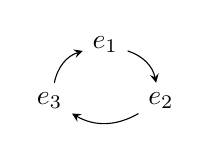
\begin{tikzpicture}[-stealth,auto]
                \node (a) {$e_1$};
                \node (b) [below right of=a] {$e_2$};
                \node (c) [below left of=a] {$e_3$};
                
                \path[every node/.style={font=\sffamily\small}]
                (a) edge [bend left] node[right] {} (b)
                (b) edge [bend left] node[right] {} (c)
                (c) edge [bend left] node[left] {} (a);
            \end{tikzpicture}
        \end{minipage}
    \end{center}
\end{prop}
\begin{proof} Tenemos que:
    \begin{equation*}
        e_1\times e_2 = \left|\begin{array}{ccc}
            e_1 & e_2 & e_3 \\
            1 & 0 & 0 \\
            0 & 1 & 0
        \end{array}\right| =
        - \left|\begin{array}{cc}
            e_1 & e_3 \\
            1 & 0 \\
        \end{array}\right|
        = e_3
    \end{equation*}
    \begin{equation*}
        e_2\times e_3 = \left|\begin{array}{ccc}
            e_1 & e_2 & e_3 \\
            0 & 1 & 0 \\
            0 & 0 & 1
        \end{array}\right| =
         \left|\begin{array}{cc}
            e_1 & e_2 \\
            0 & 1 \\
        \end{array}\right|
        = e_1
    \end{equation*}
    \begin{equation*}
        e_3\times e_1 = \left|\begin{array}{ccc}
            e_1 & e_2 & e_3 \\
            0 & 0 & 1 \\
            1 & 0 & 0
        \end{array}\right| =
         \left|\begin{array}{cc}
            e_2 & e_3 \\
            0 & 1 \\
        \end{array}\right|
        = e_2
    \end{equation*}
\end{proof}

\begin{prop}
    Sea el EVME $(V^3, g)$. Consideramos $u,v,w\in V^3$. Entonces:
    \begin{equation*}
        u\times (v \times w) = g(u,w) v - g(u,v) w
    \end{equation*}
\end{prop}
\begin{comment}
\begin{proof}
    Realizamos la siguiente distinción de casos:
    \begin{itemize}
        \item \underline{Si $v,w$ linealmente dependientes}:

        Tenemos que $w=kv,\quad k\in \bb{R}$. Entonces:
        \begin{equation*}
            0= u\times (v \times kv) = kg(u,v) v - g(u,v) kv = 0 \Longleftrightarrow 0=0 \quad\text{cierto trivialmente.}
        \end{equation*}

        \item \underline{Si $v,w$ linealmente independientes}:

        Sea $\cc{B}_o=\{e_1, e_2, e_3\}$ base ortonormal positiva, y veamos que se cumple para dicha base:
        \begin{equation*}
            e_1\times (e_2 \times e_3) = e_1\times e_1 = 0 = 0\cdot e_2 - 0\cdot e_3
        \end{equation*}
        
        Tomamos como base $\cc{B}'=\{v,w,u\}$ definida positiva (esto no es restrictivo, ya que en caso contrario se cambian de orden).
    \end{itemize}
\end{proof}
\end{comment}



\begin{prop}
    Sea el EVME $(V^3,g)$. Consideramos $u,u',v,v'\in V^3$. Entonces:
    \begin{equation*}
        g( u\times u',v\times v') = g( u,v)g( u', v') -g( u,v')g( u', v)
    \end{equation*}
\end{prop}

\begin{comment}
\begin{proof} Realizamos la siguiente distinción:
    \begin{itemize}
        \item \underline{Supuesto $u$ linealmente dependiente a $u'$}: \begin{equation*}
            g( u\times u,v\times v') = g(u,v)g(u,v') -g(u,v')g(u, v) \Longleftrightarrow g(0,v\times v') = 0 \Longleftrightarrow 0=0
        \end{equation*}
        
        \item \underline{Supuesto $u$ linealmente independiente a $u'$}:
        
        Lo demostramos para una cierta base orientada positiva $\cc{B}_o = \{u,u', e_3\}$. Entonces:
        \begin{equation*}
            g( u\times u',v\times v')
            = g( e_3,v\times v')
            = g( u,v)g( u', v') -g( u,v')g( u', v)
        \end{equation*}
    \end{itemize}
\end{proof}
\end{comment}


\begin{coro}
Sea el EVME $(V^3,g)$. Consideramos $u,u'\in V^3-\{0\}$. Entonces:
    \begin{equation*}
        \sen ^2 \theta = \frac{||u\times u'||^2}{(||u||\;||u'||)^2}
    \end{equation*}

    donde $\theta = \measuredangle \{u,u'\}$.
\end{coro}
\begin{proof}
    De la proposición anterior, tomamos $v=u, v'=u'$. Entonces:
    \begin{equation*}
        ||u\times u'||^2 = ||u||^2 ||u'||^2 - g (u,u')^2 
    \end{equation*}

    Como tenemos que $g(u,u') = ||u||\;||u'||\;\cos \theta$, se tiene lo siguiente:
    \begin{equation*}
        ||u\times u'||^2 = ||u||^2||u'||^2 - ||u||^2||u'||^2\cos ^2 \theta
        = ||u||^2||u'||^2 (1-\cos^2 \theta)
    \end{equation*}

    Usando la relación trigonométrica $\sen^2 \theta +\cos^2 \theta  = 1$, se tiene que:
    \begin{equation*}
        ||u\times u'||^2 = ||u||^2 ||u'||^2\sen ^2 \theta \Longrightarrow
        \sen ^2 \theta = \frac{||u\times u'||^2}{(||u||\;||u'||)^2}
    \end{equation*}
    donde hemos usado que $u,u'\neq 0$.
    
\end{proof}

\begin{comment}
\begin{definicion}[Ángulo orientado]
    Sean $u,v\in V^3$ linealmente independientes. Tenemos que el ángulo orientado se define como $\theta $
\end{definicion}
\end{comment}

\section{Proceso de Ortogonalización de Gram-Schmidt}

Sea $(V^n, g)$ un EVME y consideramos $\cc{B}=\{e_1, \dots, e_n\}$ una base. Vamos a construir, a partir de $\cc{B}$, una base ortogonal $\bar{\cc{B}}=\{\bar{e_1}, \dots, \bar{e_n}\}$ de $V$.

Partimos desde $\bar{e_1} = e_1$. Consideramos $\bar{e_2} = e_2 -a\bar{e_1}$, y calculamos $a\in \bb{R}$ tal que $\bar{e_1} \perp \bar{e_2}$.
\begin{equation*}
    0=g(\bar{e_2}, \bar{e_1}) = g(e_2-a\bar{e_1}, \bar{e_1})=  g(e_2, \bar{e_1}) -a ||\bar{e_1}||^2
    \Longrightarrow a = \frac{g(e_2, \bar{e_1})}{||\bar{e_1}||^2}
\end{equation*}

Posteriormente, consideramos $\bar{e_3} = e_3 -b\bar{e_1} -c\bar{e_2}$, y ajustamos $b,c\mid \bar{e_3}\perp \bar{e_1},\bar{e_2}$.

Así sucesivamente se obtiene cada vector $\bar{e_i}$, y luego se puede normalizar dicha base para obtener una base ortonormal.

\begin{ejemplo}
    Sea el EVME $(\bb{R}^4,\;\langle,\rangle)$ y consideramos el subespacio vectorial $$V\equiv x_1+x_2+x_3+x_4=0$$

    Sea $\cc{B}$ base de $V$ la siguiente:
    \begin{equation*}
        \cc{B}=\{e_1, e_2, e_3\} = \left\{
        \left(\begin{array}{c}
            1 \\ -1 \\ 0 \\ 0
        \end{array}\right),
        \left(\begin{array}{c}
            1 \\ 0 \\ -1 \\ 0
        \end{array}\right),
        \left(\begin{array}{c}
            1 \\ 0 \\ 0 \\ -1
        \end{array}\right)
        \right\}
    \end{equation*}

    Aplicamos ahora el algoritmo de Gram-Schmidt para conseguir una base ortogonal $\bar{\cc{B}} = \{\bar{e_1}, \bar{e_3}, \bar{e_3}\}$ de $V$.

    Definimos $\bar{e_1} = e_1$, y sea $\bar{e_2} = e_2-a\bar{e_1}$
    \begin{equation*}
        0 = \langle e_2, \bar{e_1}\rangle -a||\bar{e_1}||^2 = 1-2a \Longrightarrow a=\frac{1}{2}
    \end{equation*}

    Entonces, tenemos que:
    \begin{equation*}
        \bar{e_2} = e_2 -\frac{1}{2}\bar{e_1} = \frac{1}{2}\left(\begin{array}{c}
            1 \\ 1 \\ -2 \\ 0
        \end{array}\right)
    \end{equation*}

    Sea ahora $\bar{e_3} = e_3 -a\bar{e_1} -b\bar{e_2}$.
    \begin{equation*}
        \left\{\begin{array}{l}
            \bar{e_3}\perp \bar{e_1} \Longrightarrow 0=\langle e_3, \bar{e_1}\rangle - a||\bar{e_1}||^2  \\
            \bar{e_3}\perp \bar{e_2} \Longrightarrow 0=\langle e_3, \bar{e_2}\rangle - b||\bar{e_2}||^2  \\
        \end{array}\right.
    \end{equation*}

    Resolviendo ese sistema hallamos $\bar{e_3}$, y ya tenemos una base ortogonal.
\end{ejemplo}


\section{Ejercicios}
Los ejercicios resueltos del presente tema están disponibles en la sección \ref{sec:EjerciciosTema3}.